\chapter{Marco teórico}\label{cap:marcoteorico}

En este capitulo se proporciona los antecedentes y se detallan los conceptos teóricos en lo que se basa esta tesis. Empezando con la detección de objetos tradicional y sus componentes. Luego, se desarrolla el problema de aprendizaje sin ejemplos y como este se usa en la detección de objetos sin ejemplos. 

\section{El problema de detección de objetos} \label{sec:elproblemadedetcciondeobjetos}
Con los avances recientes en los modelos de visión por computadora basados en el aprendizaje profundo, las aplicaciones de detección de objetos son más fáciles de desarrollar que nunca. Además de importantes mejoras de rendimiento, estas técnicas también han aprovechado conjuntos de datos de imágenes masivos para reducir la necesidad de generar conjuntos de datos grandes. Con los enfoques actuales que se centran en arquitecturas con un pipeline de extremo a extremo, el rendimiento también ha mejorado significativamente, lo que permite casos de usos en tiempo real.\\


La detección de objetos es una importante tarea de visión por computadora, que consiste en localizar la presencia de objetos de determinadas clases, como humanos, automóviles, frutas, o animales, en imágenes digitales. El objetivo de la detección de objetos es desarrollar modelos y técnicas computacionales que proporcionen una de las piezas de información más básicas que necesitan las aplicaciones de visión por computadora: ¿Qué objetos están y dónde? En la \autoref{fig:example_detection} se muestra un ejemplo del resultado generado por estos algoritmos.\\

\begin{figure}
	\centering
	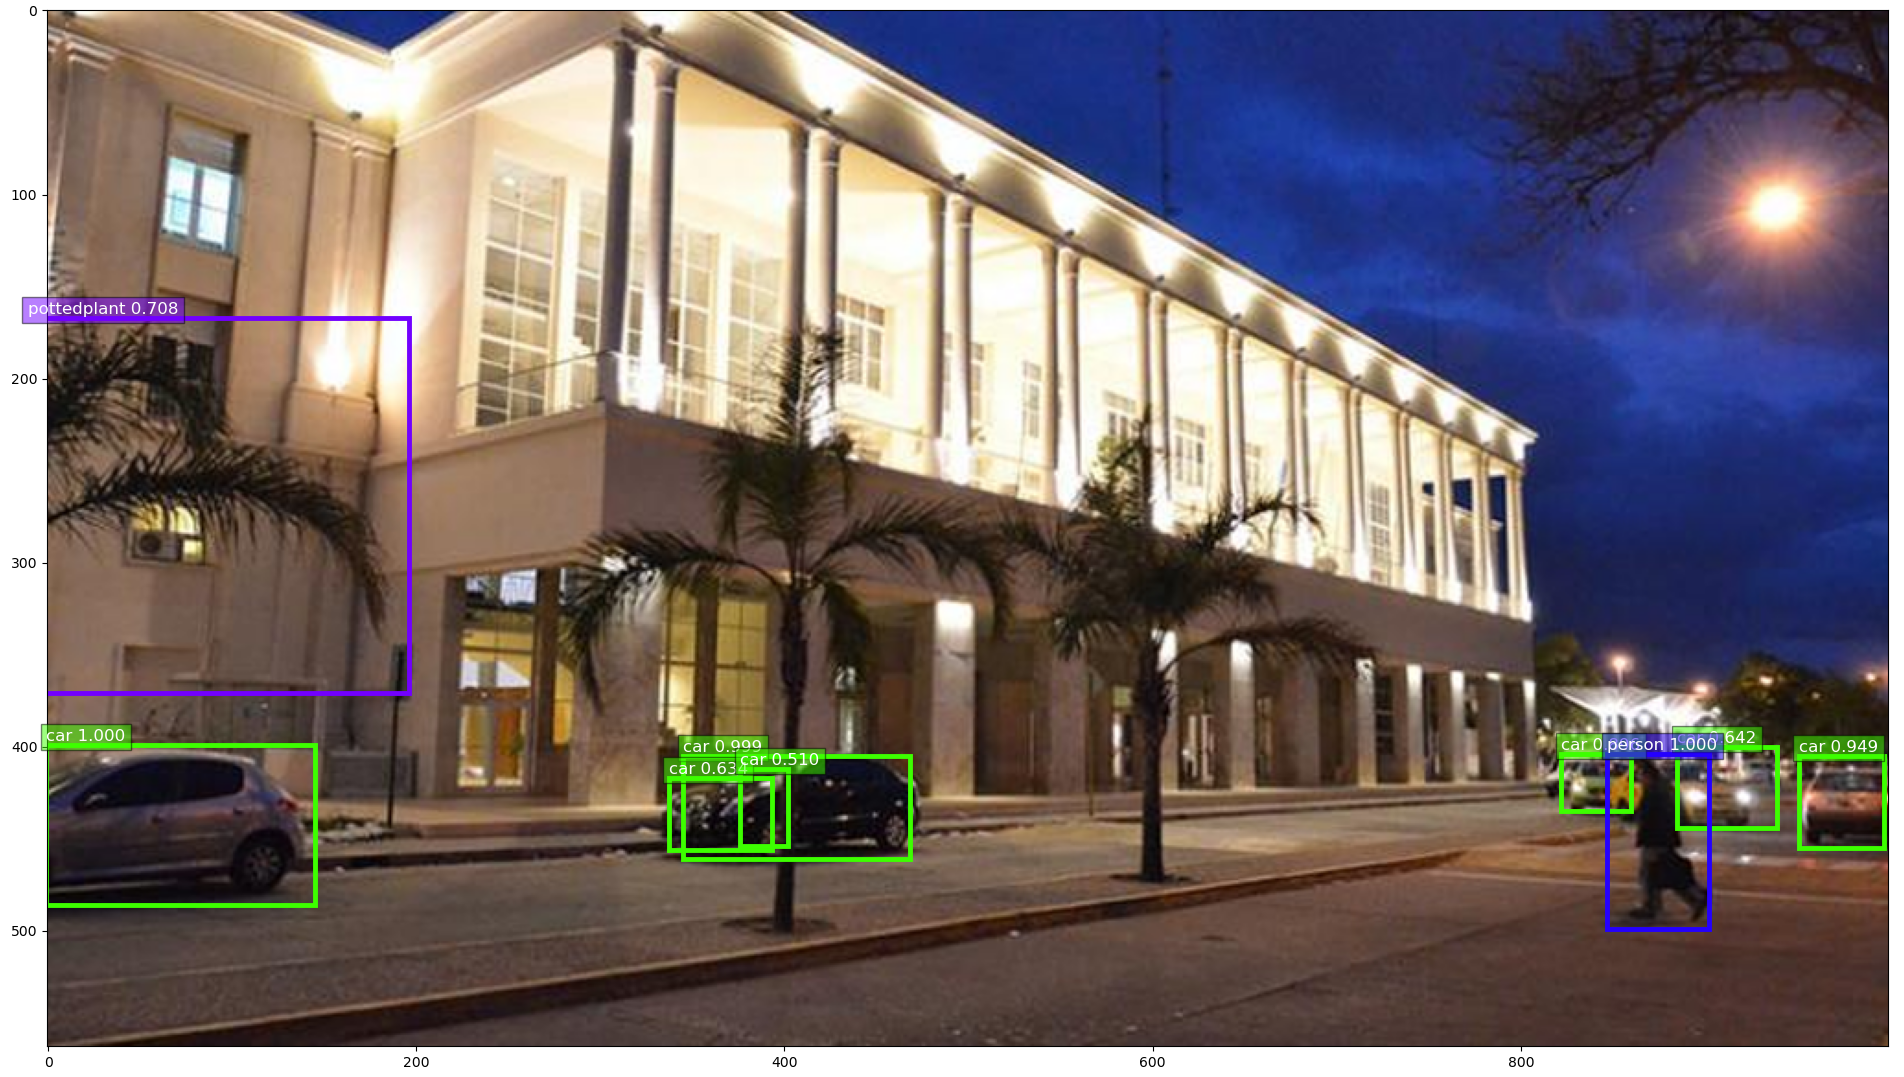
\includegraphics[width=\textwidth]{ejemplo_detecion_de_objetos.png}
	\caption{Ejemplo de detección de objetos, el modelo utilizado es Faster R-CNN~\cite{ren2015faster}. Las clases que puede detectar esta implementación son: ``Auto (\textit{car})'',  ``Persona (\textit{person})'',  ``Planta en maceta (\textit{potted plant})'', entre otras.}
	\label{fig:example_detection}
\end{figure}

Se puede considerar que la detección de objetos tiene asociado dos sub-problemas:

\begin{itemize}
	\item \textbf{Localización:} localiza la presencia de un objeto en la imagen y lo representa con un cuadro delimitador (\textit{Bounding box}). Toma una imagen como entrada y muestra la ubicación del cuadro delimitador en algún formato, por ejemplo: (posición, alto y ancho).
	\item \textbf{Reconocimiento:} tiene como entrada una sub-figura de una imagen (generalmente indicada por un cuadro delimitador) y genera la etiqueta de clase de esa figura, junto a una medida de la confianza que indica que tan ``buena'' es la predicción. Este problema esta asociado con la clasificación de imágenes, el cual genera una etiqueta y una medida de confianza para una imagen completa.
\end{itemize}


Teniendo en cuenta estos dos componentes, existen principalmente dos tipos de detectores de objetos. Por un lado, tenemos detectores de dos etapas (\textit{two-stage}), como Faster R-CNN~\cite{ren2015faster}, que utiliza una red  RPN (por su denominación en inglés \textit{region proposal network}) para generar regiones candidatas a contener un objeto de cualquier clase, y luego enviar estas propuestas a una red de reconocimiento. Estos modelos alcanzan las tasas de precisión más altas pero suelen ser más lentos. Por otro lado, tenemos detectores de una etapa (\textit{one-stage}), como YOLO~\cite{redmon2016you}, que tratan la detección de objetos como un simple problema de regresión, tomando una imagen de entrada y aprendiendo la predicción de clase y coordenadas del cuadro delimitadores en una misma red. Estos últimos tienen un diseño más eficiente y elegante. 

Los detectores de dos etapas filtran la mayoría de las propuestas negativas, pasando a la etapa de clasificación un numero menor de cuadros. Mientras que los detectores de una etapa se enfrentan directamente a todas las regiones de la imagen reduciendo su desempeño.

En este trabajo nos centraremos en detectores de objetos de dos etapas, la \autoref{fig:OneStage} muestra un ejemplo de como funcionan estos tipos de detectores.\\

\begin{figure}
	\centering
	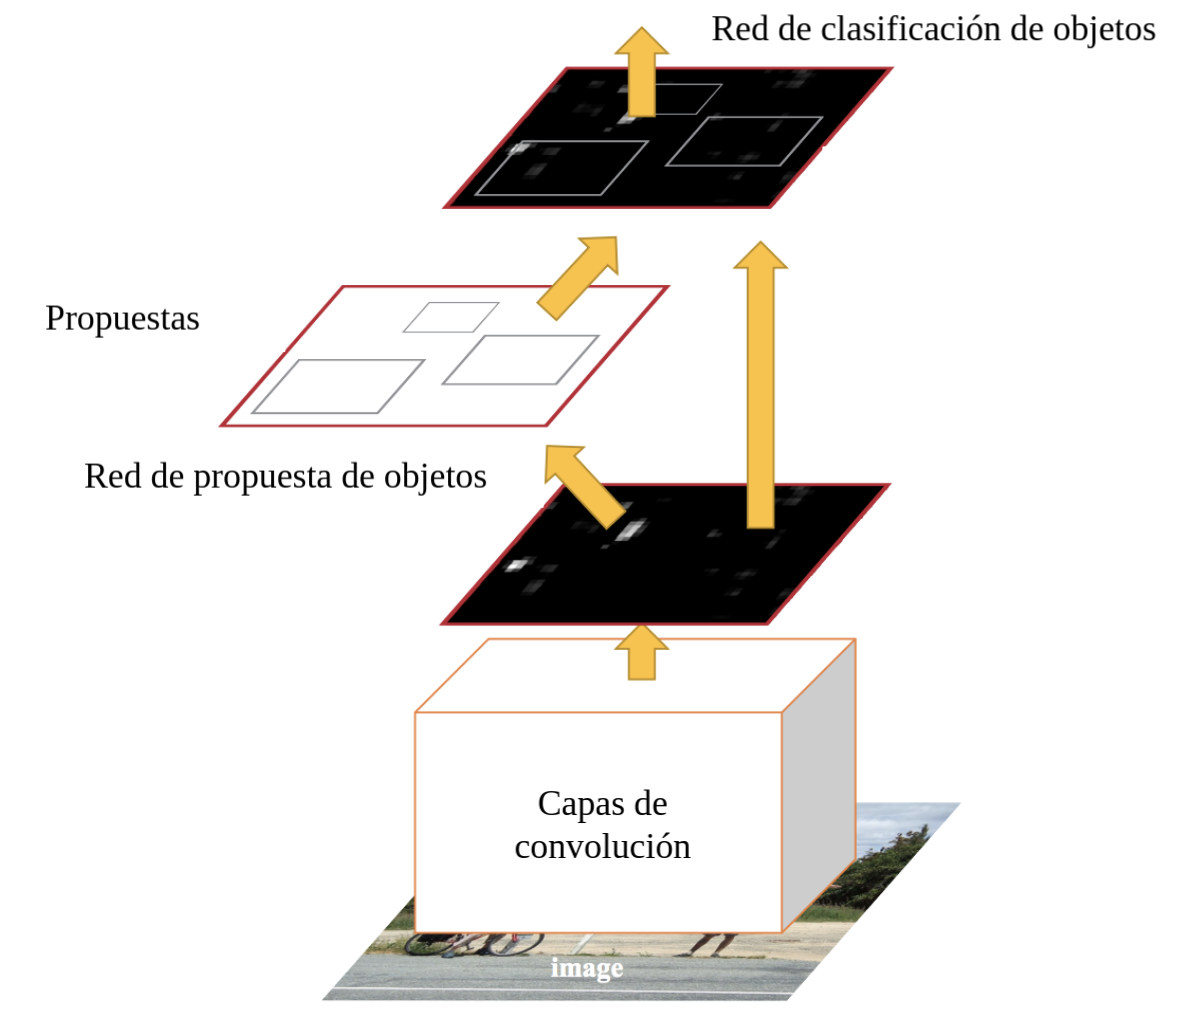
\includegraphics[width=1\textwidth]{one_stage.png}
	\caption{Las distintas etapas de un detector de objetos \textit{two-stage}. Imagen adaptada del trabajo Faster R-CNN~\cite{ren2015faster}.}
	\label{fig:OneStage}
\end{figure}

\section{Datos de entrenamiento} \label{sec:datosdeentrenamiento}
Los datos, en general, son un elemento vital de los proyectos de aprendizaje automático supervisado. Cuantos más datos tenga, mejor será el producto final. Sin embargo, no basta con tener datos brutos, sino que se deben tener estos datos anotados. Dichas anotaciones surgen del proceso de etiquetado que consiste en indicar la ``cosa'' de interés. Dependiendo de los datos y el objetivo final, esta tarea varia. Las etiquetas junto a los datos brutos, ``alimentan'' al algoritmo de aprendizaje automático que luego permiten identificar correctamente los objetos en una imagen, comprender el habla humana y muchas otras funcionalidades. La tarea de etiquetado implica un gran porcentaje del tiempo de desarrollo del proyecto de aprendizaje automático, y además, su costo es muy elevado. La razón por la que la anotación de datos es tan importante es que incluso el más mínimo error podría resultar en un modelo deficiente. Esta es una de las áreas en la que los humanos tenemos una ventaja respecto a las computadoras, ya que podemos lidiar mejor con la ambigüedad, descifrar la intención y muchos otros factores que intervienen en la anotación de datos.

Por otro lado, por lo general, las anotaciones sufren de un fenómeno denominado ``cola larga'' (o mas conocido como \textit{long tail}). Este fenómeno surge cuando  el número de ejemplos de entrenamiento por clase varía de miles, para las clases principales, a tan solo unos pocos, para las clases finales. El problema de ``cola larga'' se puede observar en los datos anotados de COCO  \autoref{fig:COCOAnotaciones}, donde la clase persona tiene aproximadamente 260.000 instancias, y otras clases, como tijeras, oso o parquímetro, tienen solo 1000 anotaciones.

En el contexto de la detección de objetos los datos anotados son cuadros delimitadores y sus etiquetas. Una pregunta que siempre se hace es la siguiente: para un modelo de detección de objetos en un problema X, ¿cuántas imágenes se necesitan? La respuesta mas común que se encuentra en la red es 1000 imágenes por clase que se quiere detectar. El origen de este número mágico, proviene del desafío de clasificación de ImageNet original, donde el conjunto de datos tenía, 1000 categorías cada una con 1000 imágenes aproximadamente y por lo general un objeto por imagen. Pero si lo comparamos con un conjunto de datos actual (COCO) donde se evalúa detección de objetos, podemos observar que se requiere muchas mas anotaciones (aproximadamente 10.000 anotaciones en promedio, ver \autoref{fig:COCOAnotaciones}).

\begin{figure}
	\centering
	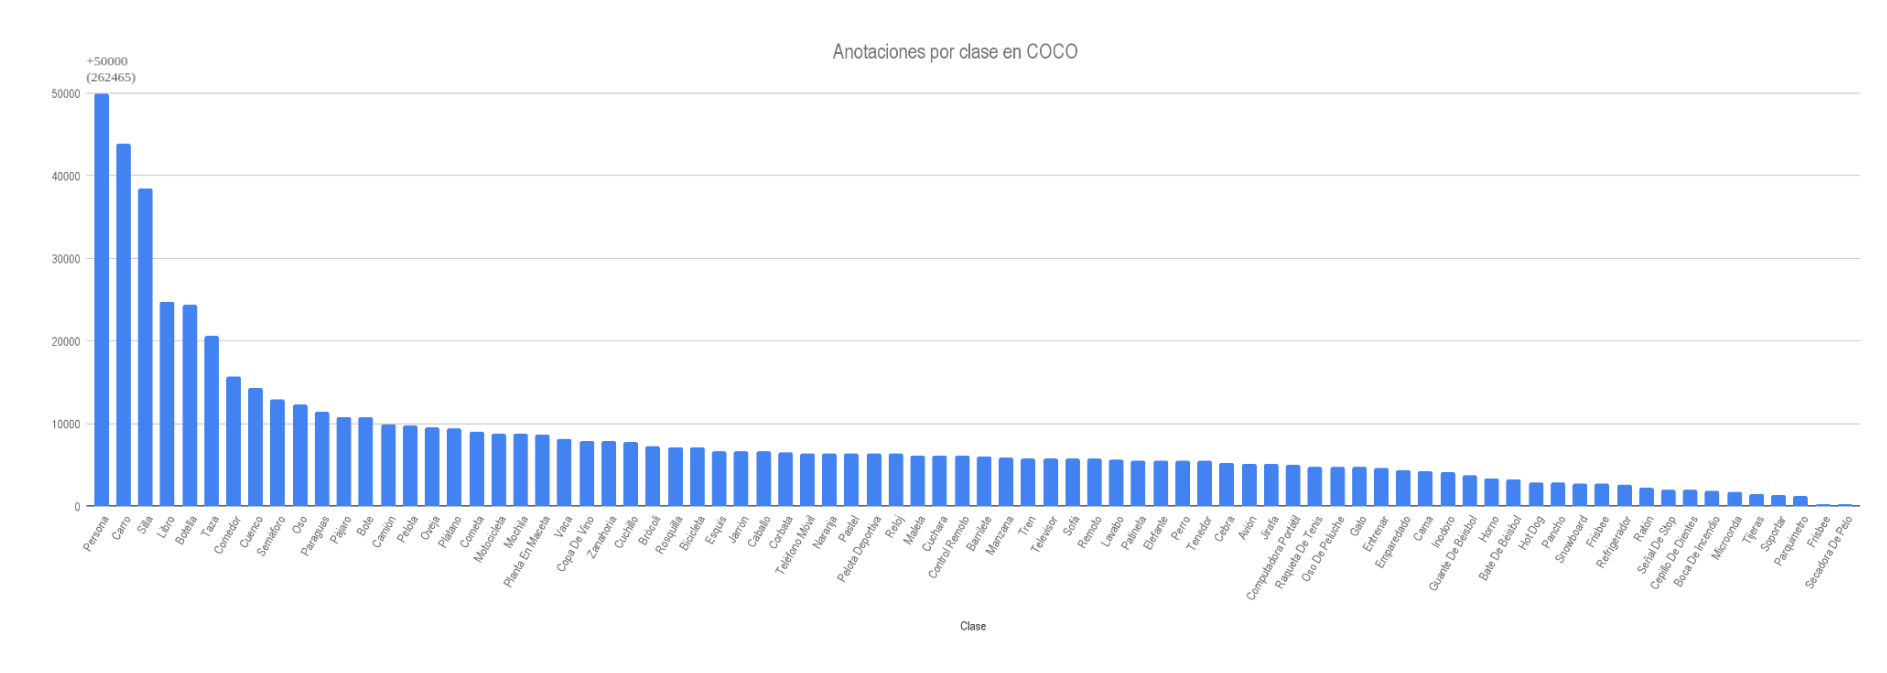
\includegraphics[width=1\textwidth]{coco_anotaciones.png}
	\caption{Numero de anotaciones por clases en el conjunto de datos COCO. TODO: TRASPONER}
	\label{fig:COCOAnotaciones}
\end{figure}

Esto ejemplos nos ayudan a orientarnos, pero dar un número exacto es difícil, ya que el número de imágenes necesarias varía mucho dependiendo del problema. Lo que se necesita es un conjunto de imágenes que representen todos los escenarios posibles en el que puede aparecer el objeto que se quiere detectar. Conseguir este conjunto puede que resulte muy difícil, ya sea por el costo que conlleva generar esas anotaciones, por que los escenarios donde aparece el objeto son demasiados, o por que simplemente es complicado conseguir una imagen del objeto.\\

Por estos motivos es necesario encontrar algún método que reduzca el numero de anotaciones necesarias para la detección de objetos. Es así como nacen los métodos denominados ``Aprendizaje sin ejemplos'', los cuales analizaremos a continuación.
 
\section{Aprendizaje sin ejemplos} \label{sec:aprendizajesinejemplos}
El Aprendizaje sin ejemplos (ZSL, por su denominación en inglés \textit{Zero-shot Learning}), es un conjunto de problemas de aprendizaje automático, donde en el momento de la prueba se observan muestras de clases que no se observaron durante el entrenamiento, y se necesita predecir la categoría a la que pertenecen. Esta se diferencia de las configuraciones estándares de aprendizaje automático, donde se espera que se clasifiquen correctamente las nuevas muestras en las clases que ya se han observado durante el entrenamiento. 

Esta técnica se puede aplicar en problemas de visión por computadora, y algunos de sus escenarios son:

\begin{itemize}
	\item \textbf{Cuando el número de clases objetivo es grande.} Generalmente, los seres humanos pueden reconocer una gran cantidad de clases. Sin embargo, recopilar suficientes instancias etiquetadas para un número tan grande de clases es un desafío.
	
	\item \textbf{Cuando las clases objetivo son raras.} Supongamos que queremos reconocer flores de diferentes especies. Es difícil recopilar suficientes instancias de imágenes para todas las especies. Además, para muchas flores raras, no podemos encontrar las instancias etiquetadas correspondientes.
	
	\item \textbf{Cuando las clases de interés cambian con el tiempo.} Un ejemplo es reconocer imágenes de productos pertenecientes a cierto estilo o marca. Dado que los estilos y marcas cambian con frecuencia, para algunos productos nuevos, es difícil encontrar los casos etiquetados correspondientes.
	
	\item \textbf{Cuando el costo de obtener las instancias etiquetadas es alto.} El proceso de etiquetado de instancias es caro y requiere mucho tiempo. Por ejemplo, supongamos que queremos detectar un animal en extinción para poder rastrearlos y tener una forma de contabilizarlos y proteger las áreas donde se encuentran, por ejemplo el yaguareté que habita el Chaco Argentino. Poder conseguir un conjunto considerable de fotos del mismo en distintos entornos, situaciones y ubicaciones, como de día, noche, corriendo, descansando, etc. puede resultar un gran desafió y demasiado tarde si conlleva mucho tiempo.
\end{itemize}

Todos estos problemas se pueden intentar solucionar con ZSL, entrenando los modelos con clases similares y luego evaluando las clases que nos interesan. Por ejemplo, para el problema del  yaguareté, se puede proponer un modelo de ZSL, entrenado con imágenes de animales similares como leopardo, puma, chita, etc., y luego utilizar este modelo para detectar el yaguareté.\\
 
Es necesario entender que en este tipo de configuración, existen dos tipos de clases. Las vistas, que son todas aquellas que tienen al menos una instancia en los datos de entretenimiento y las invisibles que no tienen ninguna instancia en los datos de entrenamiento. Dicho esto, el aprendizaje sin ejemplos se puede dividir en categorías según los datos presentes durante la fase de entrenamiento y la fase de prueba:
\begin{itemize}
	\item En base a los datos disponibles en el momento de entrenar un modelo.
	\begin{itemize}
		\item \textbf{Zero-shot learning inductivo:} se tiene acceso a los datos y a la información complementaria de solo las clases vistas.
		\item \textbf{Zero-shot learning transductivo:} además de los datos y la información complementario de las clases vistas,  se tiene acceso a los datos de las clases no vistas.
	\end{itemize}
	\item Basado en los datos disponibles en el momento de la inferencia.
	\begin{itemize}
		\item \textbf{Zero-shot learning convencional (ZSL):} en las pruebas solo se evalúan las clases no vistas.
		\item \textbf{Zero-shot learning generalizado (GZSL):} en las pruebas se evalúan tanto las clases vista como las no vistas.
	\end{itemize}
\end{itemize}

En el aprendizaje sin ejemplo, no se tiene información sobre las clases no vistas en el entrenamiento. La forma de suplir la falta de esa información sobre las clases que se quiere predecir, es utilizar otro espacio que pueda representar tanto las clases vista como las invisibles. Para poder generar ese espacio, se necesita algún tipo de información auxiliar, que pueda representar todas las clases.
Algunos ejemplos de información auxiliar son, una estructura de clases, una descripción textual en lenguaje natural, etc. La \autoref{fig:modales} muestra algunos tipos de información subsidiaria para un mismo dato de entrada.

\begin{figure}[]
	\centering
	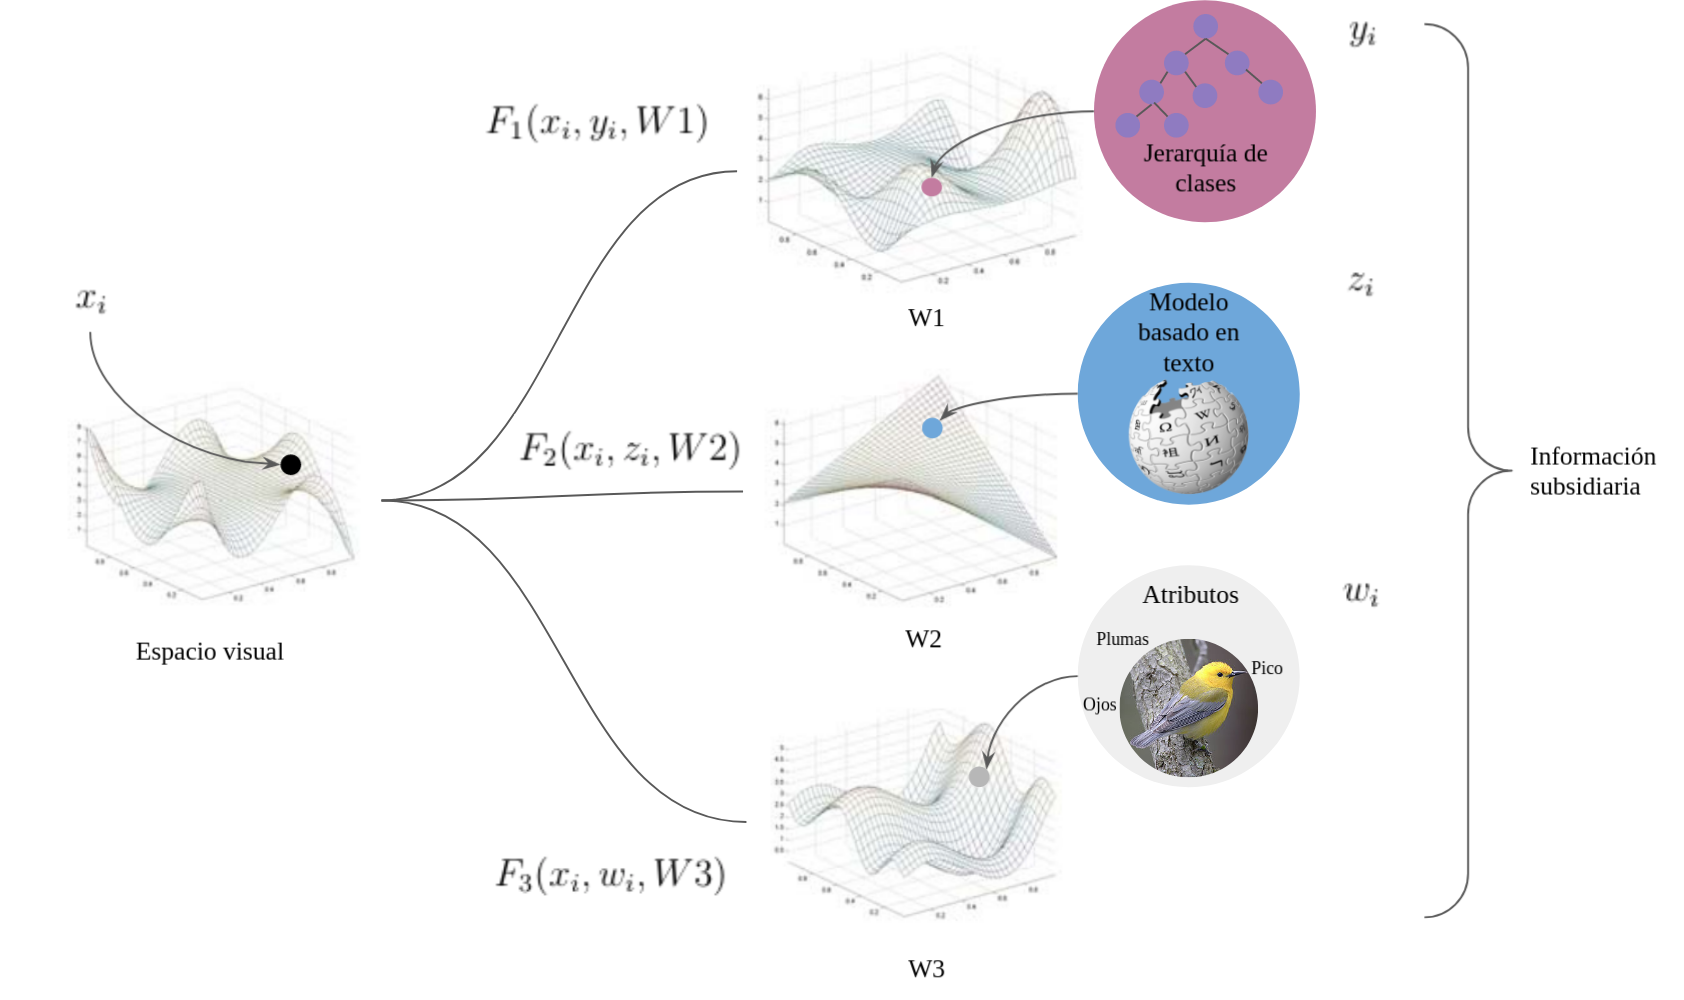
\includegraphics[width=0.8\textwidth]{img/modales.png}
	\caption{Idealización de distintos tipos de información subsidiaria con sus respectivos espacios.}
	\label{fig:modales}
\end{figure}

En obras existentes, el enfoque de información auxiliar se inspira en la forma en que los seres humanos reconocen el mundo. Los seres humanos pueden realizar un aprendizaje sin ejemplo con la ayuda de algunos conocimientos semánticos. Por ejemplo, con el conocimiento de que ``una zebra se parece a un caballo y tiene rayas'', podemos reconocer una zebra incluso sin haberla visto antes, siempre que sepamos cómo es un caballo y cómo se ve el patrón rayas. De esta manera, la información auxiliar involucrada por los métodos de aprendizaje sin ejemplos existentes suele ser información semántica que forman un espacio que contiene tanto las clases visibles como las invisibles.\\

Esta técnica de utilizar dos tipos de información, semántica y visual se denomina multimodales. La modalidad se refiere a la forma en que algo sucede o se experimenta. Un problema de investigación se caracteriza como multimodal cuando incluye datos de distinta naturaleza. La \autoref{fig:EjemploZSD} muestra un ejemplo de como funciona un clasificador sin ejemplos usando multimodales, asociando las imágenes a un vector perteneciente a un espacio que representa a todas las clases.\\

A continuación se detalla como se puede procesar y representar los dos tipos de información utilizado en este trabajo, visuales y semánticos.

\begin{figure}[]
	\centering
	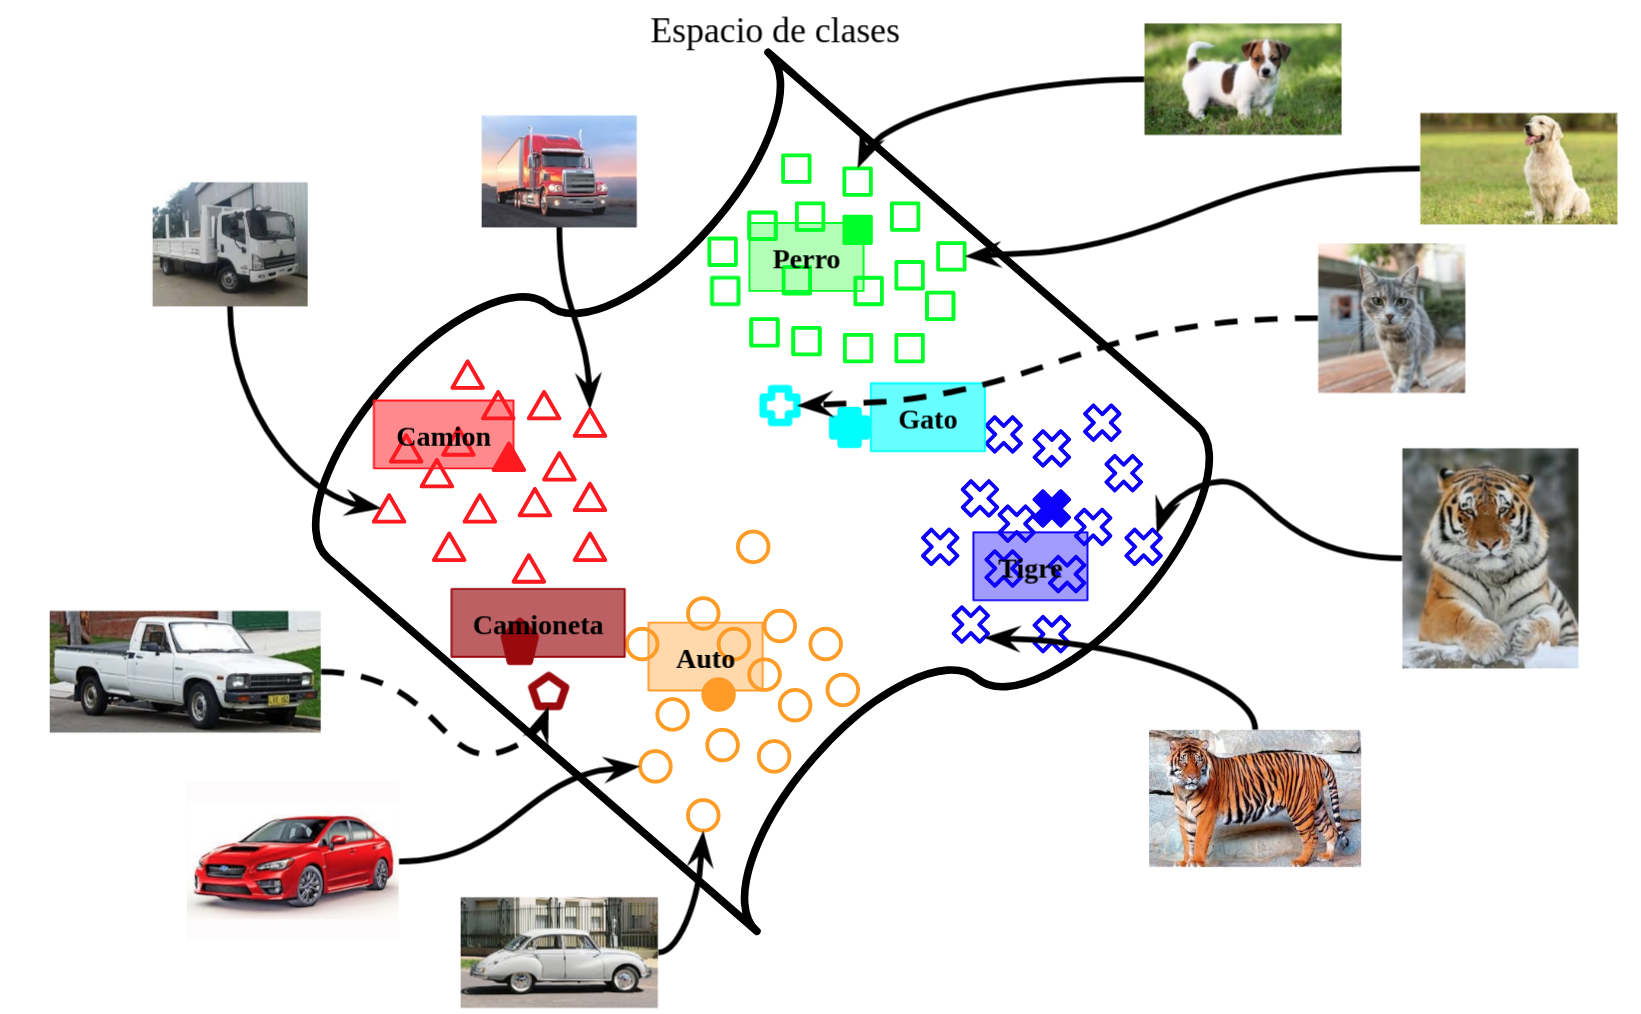
\includegraphics[width=0.8\textwidth]{img/Modelo.png}
	\caption{Descripción de como funciona un clasificador de imágenes usando aprendizaje sin ejemplo. ``Auto'', ``Camión'', ``Perro'' y ``Tigre'' se observan  durante el entrenamiento,  ``Gato'' y ``Camioneta'' son clases invisibles. El formato de las imágenes sufren una transformación y se mapean a un espacio donde se contiene la información de todas las clases. Este mapeo agrupa distintas imágenes de una clase en espacios cercanos y mientras mas distinta es la clase mas alejadas están.}
	\label{fig:EjemploZSD}
\end{figure}


\subsection{Redes neuronales convolucionales} \label{sec:redesneuronalesconvolucionales}
Las redes neuronales convolucionales, o CNN por sus siglas en inglés, son un tipo de modelos de aprendizaje profundo (\textit{Deep learning}) utilizadas  para procesar distintos tipos de datos, pero empleadas generalmente en el dominio de las imágenes. Está inspirado en la organización de la corteza visual de los animales, diseñada para aprender de forma automática y adaptativa patrones en jerarquías, de bajo a alto nivel. Es decir, de formas simples como cuadrados y círculos a formas mas complejas como autos. Esto quiere decir que las primeras capas pueden detectar lineas, curvas y se van especializando hasta llegar a capas más profundas que reconocen formas complejas como un rostro. Por lo general una red CNN se compone de tres tipos de capas: convolución, agrupación y capas completamente conectadas, como se puede ver en la \autoref{fig:CNNEjemplo}. El rol de cada capa es:

\begin{itemize}
	\item Convolución: somete los datos de entrada a un conjunto de filtros convolucionales, cada uno de los cuales activa ciertas características de los datos. Generalmente, esta acompañada de una capa de activación, que permite un entrenamiento más rápido y eficaz al asignar los valores negativos a cero y mantener los valores positivos. De esta manera, permite que solo las características activadas pasen a la siguiente capa.
	\item Agrupación: se coloca generalmente después de la capa convolucional. Su utilidad principal radica en la reducción de su entrada para la siguiente capa convolucional, reduciendo así el número de parámetros que la red necesita aprender.
	\item Capas completamente conectadas: Es la encargada de relacionar los datos de las capas anteriores y generar una salida, que por lo general es utilizada para clasificar los datos de entrada.
\end{itemize}


Algunos ejemplos de redes CNN son: VGG16~\cite{simonyan2014very} (que posee 13 capas de convolución, 5 de agrupación y una totalmente conectada) y AlexNet~\cite{krizhevsky2012imagenet} (que contiene 5 capas convolucionales, 3 capas de agrupación y 3 capas completamente conectadas).\\


\begin{figure}
	\centering
	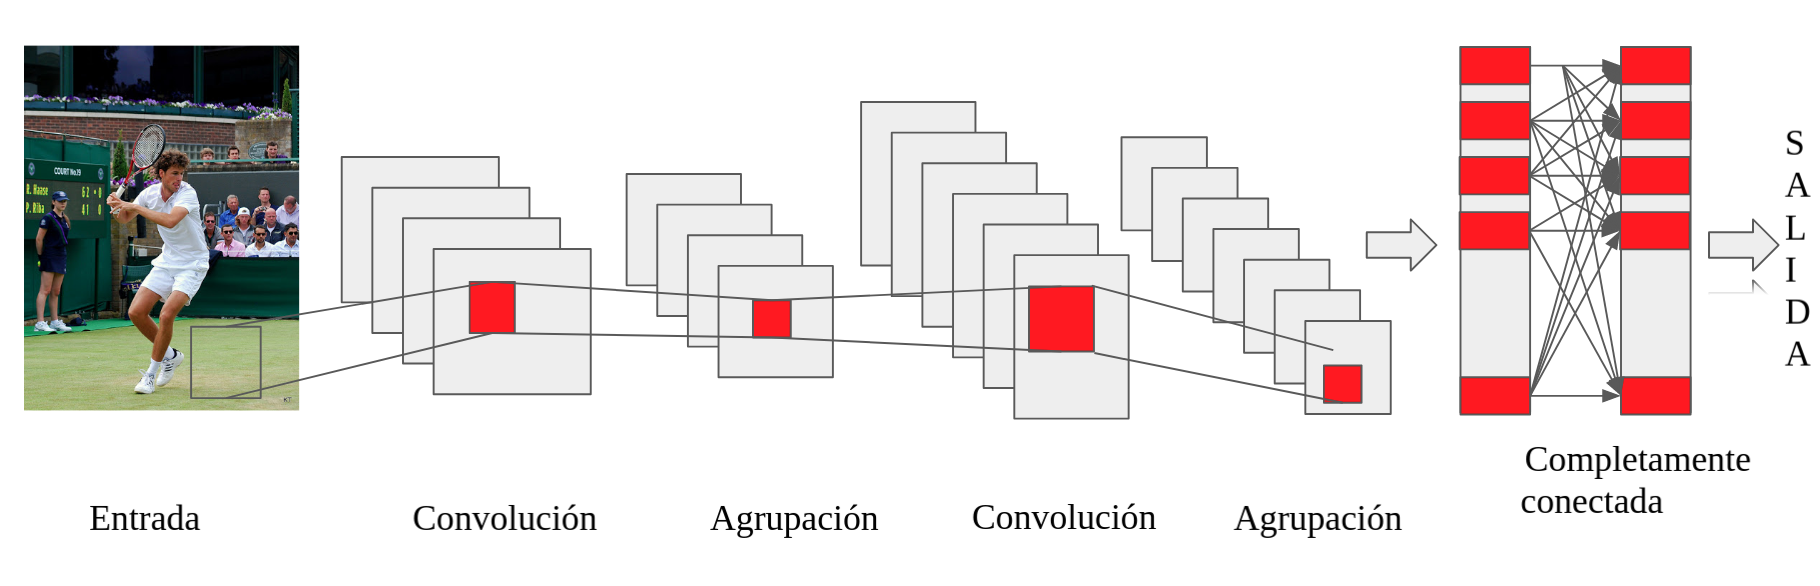
\includegraphics[width=0.9\textwidth]{img/red_cnn.png}
	\caption{Una arquitectura simplificada de una red neuronal convolucional.}
	\label{fig:CNNEjemplo}
\end{figure}

\subsection{Vectores de palabras (Word embedding)} \label{sec:wordembedding}
Así como en las imágenes utilizamos las redes CNN, para obtener un vector que represente a la misma, es necesario un procedimiento para representar clases de interés con algún objeto matemático. Hay muchas formas de representar palabras, los más usados son los \textit{word embedding}. Esta es una técnica de aprendizaje en el campo de procesamiento del lenguaje natural (PLN), capaz de capturar el contexto de una palabra en un documento, calcular similitud semántica y sintáctica con otras palabras.\\

Para entender como funcionan, consideremos las oraciones con un significado similar: ``Que tengas un buen día.'' y ``Que tengas un gran día.''. Si construimos un vocabulario exhaustivo:
\[ V = \{que, tengas, un, buen, gran, dia\}. \]
A partir de esto, se puede crear un vector codificado para cada una de estas palabras, en donde cada vector tenga el tamaño de $V$, cuyos componentes sean todos 0 excepto por el elemento en el índice que representa la palabra correspondiente en el vocabulario, que contiene un 1. Esta representación no resulta conveniente ya que la distancia entre \textit{gran} y \textit{buen} es la misma que entre \textit{tengas} y \textit{buen}.  El objetivo es que las palabras con un contexto similar ocupen posiciones espaciales cercanas. Para lograr esto, se introduce cierta dependencia de una palabra con las otras.\\

Word2Vec~\cite{mikolov2013distributed} desarrollado por Tomas Mikolov en 2013, es un modelo particularmente eficiente desde el punto de vista computacional. Este modelo se encuentra disponible de dos formas: \textit{Continuous Bag-of-Words} (CBOW) o el modelo \textit{Skip-Gram}. En CBOW, las representaciones distribuidas de contexto (o palabras circundantes) se combinan para predecir la palabra en el medio. En nuestro ejemplo \textit{gran} y \textit{buen} están rodeado de un contexto similar por lo cual resultan en vectores similares. Es varias veces más rápido de entrenar que el \textit{Skip-gram}, y tiene una precisión ligeramente mejor para las palabras frecuentes. Mientras que en el modelo \textit{Skip-gram}, la representación distribuida de la palabra de entrada se usa para predecir el contexto. Se entrena con una tarea falsa que, dada una palabra, intenta predecir las palabras vecinas. En realidad, el objetivo es solo aprender los pesos de la capa oculta que corresponden a los vectores de palabras que estamos tratando de aprender. Por ejemplo, \textit{Gran} se entrena para predecir el contexto \textit{un} y  \textit{día}, al igual que \textit{buen}. Funciona bien con una pequeña cantidad de datos de entrenamiento.

Los modelos de ZSL, aprovechan la capacidad de capturar similitudes semántica que tiene \textit{word embedding}, para relacionar las clases vistas con las clases invisibles.\\



\section{Detección de objetos sin ejemplos} \label{sec:detecciondeobjetossinejemplo}

\subsection{Introducción} 
El aprendizaje sin ejemplos identifica objetos invisibles para los que no hay imágenes de entrenamiento disponibles. Los enfoques de ZSL convencionales están restringidos a una configuración de reconocimiento donde cada imagen de prueba se clasifica en una de varias clases de objetos invisibles. Esta configuración no es adecuada para aplicaciones del mundo real donde los objetos invisibles aparecen como parte de una escena completa. Para abordar esta limitación, aparece una nueva configuración, la detección de objetos sin ejemplos ZSD (por sus siglas en ingles \textit{Zero-shot Object Detection}), que tiene como objetivo reconocer y localizar simultáneamente instancias de objetos, incluso en ausencia de ejemplos visuales de esas clases durante la fase de entrenamiento.\\

Se podría considerar que un modelo de detección de objetos sin ejemplos, es un modelo de ZSL pero con un paso extra, ubicar todas las instancias de objetos que aparecen en una imagen. Este paso se denomina propuesta de objetos y tiene que ser capas de diferenciar fondos y generar una lista con cuadros delimitadores con posibilidad de contener algún objeto. En visión artificial, la forma más popular de representar la ubicación de los objetos es con la ayuda de cuadros delimitadores (\textit{Bounding Boxes}). Existen muchos algoritmos y redes que intenta resolver este problema, algunos ejemplos son ventana deslizante (\textit{slide window}), Edge-Boxes~\cite{zitnick2014edge} y búsqueda selectiva (\textit{selective search})~\cite{uijlings2013selective}. En ZSD la propuesta de objetos cumple un papel importante, ya que se necesita extraer todas las instancias de los objetos, pero también tiene que discriminar fondos como cielo, ciudades, veredas, etc.\\ 

\begin{figure}[]
	\centering
	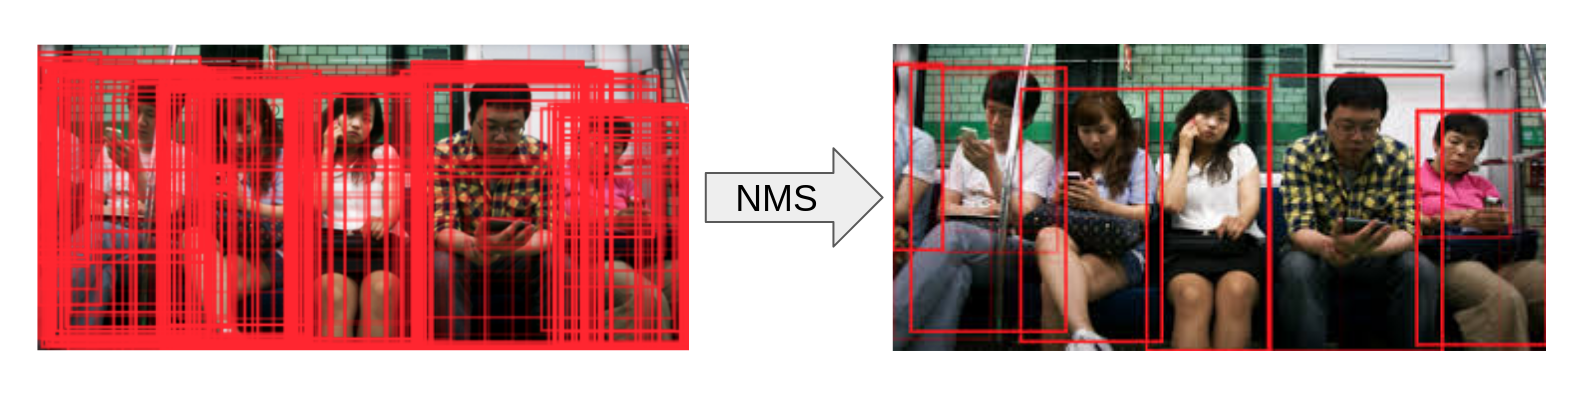
\includegraphics[width=1\textwidth]{img/NMS.png}
	\caption{Salida de un generador de propuesta de objetos y el resultado después de  usar NMS.}
	\label{fig:NMS}
\end{figure}

Como veremos en el \autoref{cap:experimentos}, en este trabajo se experimentó con Edge-Boxes~\cite{zitnick2014edge} y \textit{selective search})~\cite{uijlings2013selective}, ya que estos generan una cantidad de propuestas significativamente menor a algoritmos del estilo de ventana deslizante. Esto se debe a que no recorren toda la imagen generando distintos cuadros para distinto tamaños, sino que extraen algún tipo de información de la imagen y generan los cuadros basándose en dicha información, refinando y reduciendo el numero de cuadros. En el caso de Edge-Boxes~\cite{zitnick2014edge} se utiliza un método para generar propuestas de cuadro delimitador utilizando bordes, que proporcionan una representación escasa pero informativa de una imagen. La principal observación es que el número de contornos que están totalmente contenidos en un cuadro delimitador es indicativo de la probabilidad de que el cuadro contenga un objeto. De esta maneara con 1.000 cuadros pueden detectar hasta el 90\% de los objetos. Por otro lado, \textit{selective search}~\cite{uijlings2013selective} combina los beneficios de la búsqueda exhaustiva y de la segmentación, que agrupa los pixeles en segmentos, ya sea por color, texturas, etc. Este algoritmo genera aproximadamente 10.000 propuestas que detecta hasta el 99\% de los objetos.

Aún así, Edge-Boxes~\cite{zitnick2014edge} y \textit{selective search}~\cite{uijlings2013selective}, siguen generando una cantidad considerable de cuadros (del orden de los miles) y además, muchos cuadros con una gran superposición. Esto da lugar a una técnica de refinamiento denominada supresión de no máximos (NMS), ejemplificada en la~\autoref{fig:NMS}. La salida de NMS es un conjunto más reducido de propuestas, en la cual se filtraron todas las que se consideran repetidas y retorna solo las más representativas.\\

El requisito estricto de no utilizar ninguna imagen de clase invisible durante el entrenamiento es una condición difícil. Además, existen otras dificultades en la tarea de ZSD relacionadas al conjunto de datos de entrenamiento y prueba, es decir entre las clases vistas e invisibles. Estas dificultades son:

\begin{itemize}
	\item \textbf{Rareza}: los conjuntos de datos, por lo general, contiene un problema de distribución, es decir, muchas clases raras tienen menos cantidad de instancias. Este problema hace que las clases con mayor cantidad de instancias sesguen el modelo y las clases más raras sean marcadas incorrectamente en la etapa de prueba. Esto es un problema al momento de comparar dos modelos que fueron entrenados con distintas clases, ya que algunas separaciones de las clases resultan mejores que otras.
	
	\item \textbf{Tamaño del objeto}: algunas clases de objetos raros (tijeras, lápices, celulares, etc.), suelen tener un tamaño pequeño. Los objetos más pequeños son difíciles de detectar y reconocer. También, tienen el problema de que por lo general están junto a objetos más grandes como una mesa o una persona y se ven opacadas por estas clases.
	
	\item \textbf{Diversidad}: cuando una clase invisible no tiene otras clases visualmente similares, resulta muy difícil aprender el aspecto visual de esta. Por ejemplo, ``auto'' tiene muchas clases similares en comparación con ``cartel''. Esto permite una descripción visual inadecuada de la clase invisible ``cartel'' que eventualmente afectará el rendimiento de ZSD, a diferencia de lo que sucede con la clase ``auto''.
	
	\item \textbf{Ruido en el espacio semántico}: cuando se utiliza los vectores de incrustación semántica no supervisados como Word2Vec~\cite{mikolov2013distributed} o GloVe~\cite{pennington2014glove}, las embeddings resultante en general son ruidosas, ya que se generan automáticamente a partir de la minería de texto no anotado. Esto también afecta significativamente el rendimiento de ZSD.
\end{itemize}

\subsection{Trabajos recientes en ZSD} \label{ssec:trabajosrecientesenzsd}

Existen muchas técnicas propuestas para resolver ZSD. Cuando se empezó a leer sobre este tema a fines del 2018, la más utilizada consistía en crear una combinación de aspectos visuales y semánticos de cada objeto. Puntualmente existían tres trabajos en paralelos con una metodología similar. Bansal \etal~\cite{bansal2018zero} propuso un enfoque basado en características donde las propuestas de objetos se generan mediante edge-box. Zhu \etal~\cite{zhu2018zero} propone un método basado en el detector YOLO~\cite{redmon2016you}. Rahman \etal~\cite{rahman2018zero} propuso una extensión de Faster R-CNN~\cite{ren2015faster} junto a un nuevo enfoque transductivo para asociar objetos novedosos en el espacio semántico.\\

En los últimos dos años se publicaron nuevos trabajos utilizando esta técnica. Rahman \etal~\cite{rahman2020zero} que mejora los modelos y resultados de su trabajo previo~\cite{rahman2018zero}. Gupta \etal~\cite{gupta2020multi} donde combina predicciones obtenidas en dos espacios de búsqueda diferentes, es decir, del espacio semántico al visual, y viceversa. Rahman \etal~\cite{rahman2020improved} proponen  una función de pérdida novedosa que maneja el desequilibrio de clases y busca alinear adecuadamente los vectores visuales y semánticos.

Este trabajo se basa en el artículo científico de Bansal \etal ~\cite{bansal2018zero}, además utiliza muchos conceptos sobre zero-shot learning generalizado~\cite{zero-shot-generalizado}. Se propone un modelo zero-shot  inductivo, es decir, solo se observan imágenes de clases vistas y etiquetas que indican a que clase pertenece. Estas etiquetas son palabras del lenguaje natural sin ninguna estructura. Luego, se puede inferir todas las clases o solo las invisibles, dependiendo de si se quiere el evaluar aprendizaje por zero-shot  generalizado o convencional, respectivamente.\\ 

\subsection{Formalización de ZSD} \label{ssec:formalizaciondezsd}
Para formalizar ZSD denotamos el conjunto de las clases como $\mathcal{C} = \mathcal{S} \cup \mathcal{U}$, donde $\mathcal{S}$ son las clases vistas para entrenamiento y $\mathcal{U}$ las clases no vistas, utilizadas en la etapa de pruebas. Además se tiene que $\mathcal{S} \cap \mathcal{U} = \emptyset$. Aunque no es necesario definir el conjunto de clases de pruebas, ya que el modelo tiene que ser capás de detectar tanto clases vista como las no vista, esto se hace para poder tener una evaluación cuantitativa.

Denotamos a una imagen como $\mathcal{I} \in \mathbb{D}^{\mathcal{H} \times \mathcal{W} \times 3}$. Donde $\mathbb{D} = \{0,...,255\}$, $\mathcal{H}$  es el largo de la imagen, $\mathcal{W}$ el ancho. Esta es la forma en la que se representa cada pixel de la imagen en el formato \textbf{RGB}, donde se tiene 3 canales que caracterizan la intensidad de los colores rojo, verde y azul. 

Por cada imagen se provee un conjunto de cuadros delimitadores $\mathbb{B} = \{b_0,...,b_k\mid b_i \in N^4\}$ (cada $b_i$ representa las coordenadas de un cuadro) y sus etiquetas asociadas como $\mathbb{Y} = \{y_0,...,y_k\mid y_i \in \mathcal{C}\}$. Para cada cuadro delimitador $b_i$ extraemos una característica profunda utilizando una red neuronal convolucional denotada como $\phi(b_i) \in \mathbb{R}^{D_1}$. 

Denotamos las incrustaciones semánticas $w_j \in \mathbb{R}^{D_2}$ obtenido por algún modelo como Word2Vec~\cite{mikolov2013distributed}. El conjunto de todas las imágenes de entrenamiento se indica con $\mathcal{X}^s$, que contiene ejemplos de todas las clases de objetos visibles.  El conjunto de todas las imágenes de prueba que contienen muestras de clases de objetos invisibles se indica con  $\mathcal{X}^u$. En particular, no hay ningún objeto de clase invisible en $\mathcal{X}^s$, pero $\mathcal{X}^u$ puede contener objetos vistos.\\

El objetivo es encontrar una matriz de proyección $W_p$, tal que 
\[ \psi_i = W_p\phi(b_i) \:\:\:,\:\:\: W_P \in \mathbb{R}^{D_2 \times D_1},\:\:\: \psi_i \in \mathbb{R}^{D_2} \] 
Note que $\psi_i$ y las incrustaciones semánticas se encuentran en el mismo dominio. Como mencionamos en secciones anteriores, el espacio vectorial semántico, tiene una gran capacidad de capturar similitudes semánticas. Por lo cual, resulta clave encontrar una matriz que para cada cuadro delimitador se proyecte lo más cerca posible a la incrustación semántica de su clase. 

El resultado es una función 
\[f : \mathcal{X}, W_p  \to \{y_0,...,y_k\mid y_i \in \mathcal{C}\} \quad \operatorname{con}\quad \mathcal{X} =  \mathcal{X}^s \cup \mathcal{X}^u\] 
con un riesgo empírico regularizado mínimo $\mathcal{R}$ definido de la siguiente manera: 
\[ \arg_{}\min_{f \in F} \mathcal{R}(f(x,W_p))\quad, \] 
donde $x \in \mathcal{X}^s$ durante el entrenamiento. La función de mapeo utilizada en la etapa de inferencia, tiene la siguiente forma \[ f(x,W_p) = \arg_{}\max_{y \in \mathcal{C}}\max_{b \in \mathbb{B}(x)} (F(x,y,b,W_p)) \quad,\] donde los $\mathbb{B}(x)$ es el conjunto de propuestas de la imagen $x$. Intuitivamente se buscan los cuadros delimitadores de mejor puntuación y se les asigna la categoría de objeto de puntuación máxima.\\

Ahora que tenemos una idea general del problema de ZSD y como se define formalmente, podemos proponer una arquitectura para resolver este problema, como así también, donde y como se puede evaluar dicha arquitectura. Estos temas serán tratados en el siguiente capítulo.